\documentclass{standalone}
\usepackage{tikz}
\usetikzlibrary{patterns, positioning}


\begin{document}
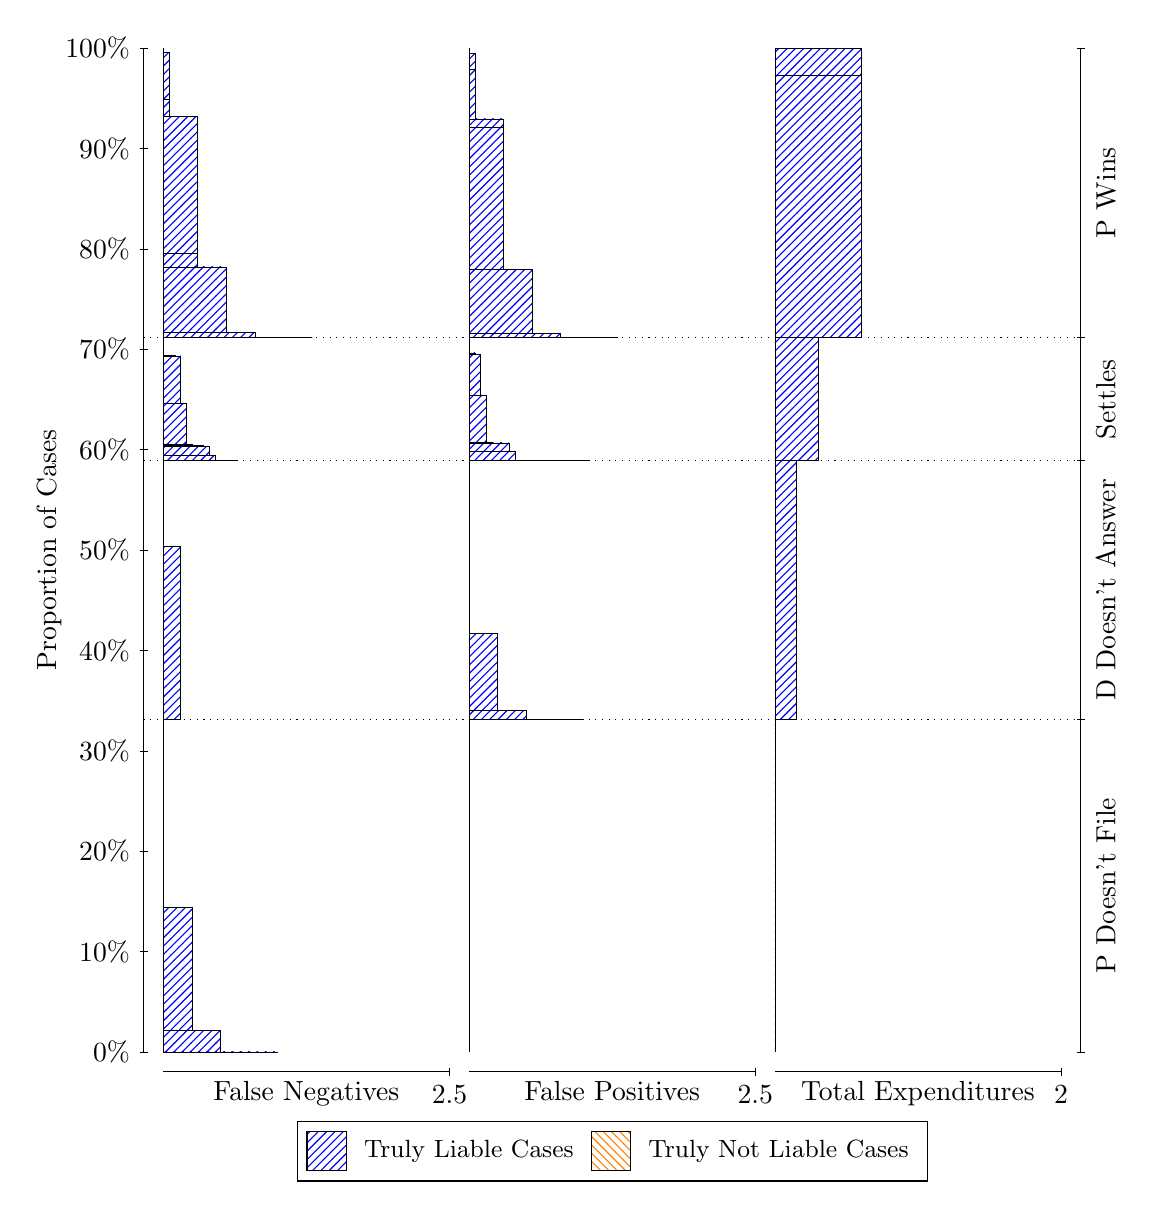
\begin{tikzpicture}
\draw[black, very thin] (1.5,1.75) -- (1.5,14.5);
\node[rotate=90, text=black, anchor=center] at (0.3, 8.125) {Proportion of Cases};
\draw[black, very thin] (1.45,1.75) -- (1.55,1.75);
\node[text=black, anchor=east] at (1.45, 1.75) {0\%};
\draw[black, very thin] (1.45,3.025) -- (1.55,3.025);
\node[text=black, anchor=east] at (1.45, 3.025) {10\%};
\draw[black, very thin] (1.45,4.3) -- (1.55,4.3);
\node[text=black, anchor=east] at (1.45, 4.3) {20\%};
\draw[black, very thin] (1.45,5.575) -- (1.55,5.575);
\node[text=black, anchor=east] at (1.45, 5.575) {30\%};
\draw[black, very thin] (1.45,6.85) -- (1.55,6.85);
\node[text=black, anchor=east] at (1.45, 6.85) {40\%};
\draw[black, very thin] (1.45,8.125) -- (1.55,8.125);
\node[text=black, anchor=east] at (1.45, 8.125) {50\%};
\draw[black, very thin] (1.45,9.4) -- (1.55,9.4);
\node[text=black, anchor=east] at (1.45, 9.4) {60\%};
\draw[black, very thin] (1.45,10.675) -- (1.55,10.675);
\node[text=black, anchor=east] at (1.45, 10.675) {70\%};
\draw[black, very thin] (1.45,11.95) -- (1.55,11.95);
\node[text=black, anchor=east] at (1.45, 11.95) {80\%};
\draw[black, very thin] (1.45,13.225) -- (1.55,13.225);
\node[text=black, anchor=east] at (1.45, 13.225) {90\%};
\draw[black, very thin] (1.45,14.5) -- (1.55,14.5);
\node[text=black, anchor=east] at (1.45, 14.5) {100\%};

\draw[black, very thin] (13.4,1.75) -- (13.4,14.5);
\draw[black, very thin] (13.35,1.75) -- (13.45,1.75);
\node[anchor=west] at (13.35, 1.75) {};
\draw[black, very thin] (13.35,5.974) -- (13.45,5.974);
\node[anchor=west] at (13.35, 5.974) {};
\draw[black, very thin] (13.35,9.2591) -- (13.45,9.2591);
\node[anchor=west] at (13.35, 9.2591) {};
\draw[black, very thin] (13.35,10.822) -- (13.45,10.822);
\node[anchor=west] at (13.35, 10.822) {};
\draw[black, very thin] (13.35,14.5) -- (13.45,14.5);
\node[anchor=west] at (13.35, 14.5) {};

\draw[black, very thin, pattern color=blue, pattern=north east lines] (1.75,1.75) rectangle (3.2033,1.75);
\draw[black, very thin, pattern color=blue, pattern=north east lines] (1.75,1.75) rectangle (2.84,1.7523);
\draw[black, very thin, pattern color=blue, pattern=north east lines] (1.75,1.7523) rectangle (2.4767,2.0232);
\draw[black, very thin, pattern color=blue, pattern=north east lines] (1.75,2.0232) rectangle (2.1133,3.587);
\draw[black, very thin, pattern color=orange, pattern=north west lines] (1.75,3.587) rectangle (1.75,3.587);
\draw[black, very thin, pattern color=blue, pattern=north east lines] (1.75,3.587) rectangle (1.75,5.974);
\draw[black, very thin, pattern color=blue, pattern=north east lines] (1.75,5.974) rectangle (1.968,8.1683);
\draw[black, very thin, pattern color=orange, pattern=north west lines] (1.75,8.1683) rectangle (1.75,8.1683);
\draw[black, very thin, pattern color=blue, pattern=north east lines] (1.75,8.1683) rectangle (1.75,9.2591);
\draw[black, very thin, pattern color=blue, pattern=north east lines] (1.75,9.2591) rectangle (2.6947,9.2594);
\draw[black, very thin, pattern color=blue, pattern=north east lines] (1.75,9.2594) rectangle (2.404,9.3268);
\draw[black, very thin, pattern color=blue, pattern=north east lines] (1.75,9.3268) rectangle (2.3313,9.4403);
\draw[black, very thin, pattern color=blue, pattern=north east lines] (1.75,9.4403) rectangle (2.2587,9.4546);
\draw[black, very thin, pattern color=blue, pattern=north east lines] (1.75,9.4546) rectangle (2.1133,9.474);
\draw[black, very thin, pattern color=blue, pattern=north east lines] (1.75,9.474) rectangle (2.0407,9.9893);
\draw[black, very thin, pattern color=blue, pattern=north east lines] (1.75,9.9893) rectangle (1.968,10.589);
\draw[black, very thin, pattern color=blue, pattern=north east lines] (1.75,10.589) rectangle (1.8953,10.595);
\draw[black, very thin, pattern color=orange, pattern=north west lines] (1.75,10.595) rectangle (1.75,10.595);
\draw[black, very thin, pattern color=blue, pattern=north east lines] (1.75,10.595) rectangle (1.75,10.822);
\draw[black, very thin, pattern color=blue, pattern=north east lines] (1.75,10.822) rectangle (3.6393,10.822);
\draw[black, very thin, pattern color=blue, pattern=north east lines] (1.75,10.822) rectangle (3.276,10.823);
\draw[black, very thin, pattern color=blue, pattern=north east lines] (1.75,10.823) rectangle (2.9127,10.884);
\draw[black, very thin, pattern color=blue, pattern=north east lines] (1.75,10.884) rectangle (2.5493,11.721);
\draw[black, very thin, pattern color=blue, pattern=north east lines] (1.75,11.721) rectangle (2.186,11.89);
\draw[black, very thin, pattern color=blue, pattern=north east lines] (1.75,11.89) rectangle (2.186,13.633);
\draw[black, very thin, pattern color=blue, pattern=north east lines] (1.75,13.633) rectangle (1.8227,13.853);
\draw[black, very thin, pattern color=blue, pattern=north east lines] (1.75,13.853) rectangle (1.8227,14.442);
\draw[black, very thin, pattern color=orange, pattern=north west lines] (1.75,14.442) rectangle (1.75,14.442);
\draw[black, very thin, pattern color=blue, pattern=north east lines] (1.75,14.442) rectangle (1.75,14.5);
\draw[black, very thin, pattern color=orange, pattern=north west lines] (5.6333,1.75) rectangle (5.6333,1.75);
\draw[black, very thin, pattern color=blue, pattern=north east lines] (5.6333,1.75) rectangle (5.6333,5.974);
\draw[black, very thin, pattern color=orange, pattern=north west lines] (5.6333,5.974) rectangle (7.0867,5.974);
\draw[black, very thin, pattern color=blue, pattern=north east lines] (5.6333,5.974) rectangle (7.0867,5.974);
\draw[black, very thin, pattern color=blue, pattern=north east lines] (5.6333,5.974) rectangle (6.7233,5.9742);
\draw[black, very thin, pattern color=blue, pattern=north east lines] (5.6333,5.9742) rectangle (6.36,6.0897);
\draw[black, very thin, pattern color=blue, pattern=north east lines] (5.6333,6.0897) rectangle (5.9967,7.0648);
\draw[black, very thin, pattern color=blue, pattern=north east lines] (5.6333,7.0648) rectangle (5.6333,9.2591);
\draw[black, very thin, pattern color=orange, pattern=north west lines] (5.6333,9.2591) rectangle (7.1593,9.2591);
\draw[black, very thin, pattern color=blue, pattern=north east lines] (5.6333,9.2591) rectangle (7.1593,9.2591);
\draw[black, very thin, pattern color=orange, pattern=north west lines] (5.6333,9.2591) rectangle (7.014,9.2591);
\draw[black, very thin, pattern color=blue, pattern=north east lines] (5.6333,9.2591) rectangle (7.014,9.2591);
\draw[black, very thin, pattern color=orange, pattern=north west lines] (5.6333,9.2591) rectangle (6.8687,9.2591);
\draw[black, very thin, pattern color=blue, pattern=north east lines] (5.6333,9.2591) rectangle (6.8687,9.2591);
\draw[black, very thin, pattern color=blue, pattern=north east lines] (5.6333,9.2591) rectangle (6.796,9.2591);
\draw[black, very thin, pattern color=blue, pattern=north east lines] (5.6333,9.2591) rectangle (6.6507,9.2591);
\draw[black, very thin, pattern color=orange, pattern=north west lines] (5.6333,9.2591) rectangle (6.578,9.2591);
\draw[black, very thin, pattern color=blue, pattern=north east lines] (5.6333,9.2591) rectangle (6.578,9.2594);
\draw[black, very thin, pattern color=blue, pattern=north east lines] (5.6333,9.2594) rectangle (6.5053,9.2595);
\draw[black, very thin, pattern color=blue, pattern=north east lines] (5.6333,9.2595) rectangle (6.4327,9.2595);
\draw[black, very thin, pattern color=blue, pattern=north east lines] (5.6333,9.2595) rectangle (6.2873,9.2596);
\draw[black, very thin, pattern color=blue, pattern=north east lines] (5.6333,9.2596) rectangle (6.2147,9.3732);
\draw[black, very thin, pattern color=blue, pattern=north east lines] (5.6333,9.3732) rectangle (6.142,9.4855);
\draw[black, very thin, pattern color=blue, pattern=north east lines] (5.6333,9.4855) rectangle (6.0693,9.4863);
\draw[black, very thin, pattern color=blue, pattern=north east lines] (5.6333,9.4863) rectangle (5.924,9.4921);
\draw[black, very thin, pattern color=blue, pattern=north east lines] (5.6333,9.4921) rectangle (5.8513,10.092);
\draw[black, very thin, pattern color=blue, pattern=north east lines] (5.6333,10.092) rectangle (5.7787,10.607);
\draw[black, very thin, pattern color=blue, pattern=north east lines] (5.6333,10.607) rectangle (5.706,10.627);
\draw[black, very thin, pattern color=blue, pattern=north east lines] (5.6333,10.627) rectangle (5.6333,10.822);
\draw[black, very thin, pattern color=orange, pattern=north west lines] (5.6333,10.822) rectangle (7.5227,10.822);
\draw[black, very thin, pattern color=blue, pattern=north east lines] (5.6333,10.822) rectangle (7.5227,10.822);
\draw[black, very thin, pattern color=orange, pattern=north west lines] (5.6333,10.822) rectangle (7.1593,10.822);
\draw[black, very thin, pattern color=blue, pattern=north east lines] (5.6333,10.822) rectangle (7.1593,10.823);
\draw[black, very thin, pattern color=orange, pattern=north west lines] (5.6333,10.823) rectangle (6.796,10.823);
\draw[black, very thin, pattern color=blue, pattern=north east lines] (5.6333,10.823) rectangle (6.796,10.88);
\draw[black, very thin, pattern color=orange, pattern=north west lines] (5.6333,10.88) rectangle (6.4327,10.88);
\draw[black, very thin, pattern color=blue, pattern=north east lines] (5.6333,10.88) rectangle (6.4327,11.689);
\draw[black, very thin, pattern color=blue, pattern=north east lines] (5.6333,11.689) rectangle (6.0693,13.493);
\draw[black, very thin, pattern color=orange, pattern=north west lines] (5.6333,13.493) rectangle (6.0693,13.493);
\draw[black, very thin, pattern color=blue, pattern=north east lines] (5.6333,13.493) rectangle (6.0693,13.601);
\draw[black, very thin, pattern color=blue, pattern=north east lines] (5.6333,13.601) rectangle (5.706,14.233);
\draw[black, very thin, pattern color=blue, pattern=north east lines] (5.6333,14.233) rectangle (5.706,14.438);
\draw[black, very thin, pattern color=blue, pattern=north east lines] (5.6333,14.438) rectangle (5.6333,14.5);
\draw[black, very thin, pattern color=orange, pattern=north west lines] (9.5167,1.75) rectangle (9.5167,1.75);
\draw[black, very thin, pattern color=blue, pattern=north east lines] (9.5167,1.75) rectangle (9.5167,5.974);
\draw[black, very thin, pattern color=orange, pattern=north west lines] (9.5167,5.974) rectangle (9.7892,5.974);
\draw[black, very thin, pattern color=blue, pattern=north east lines] (9.5167,5.974) rectangle (9.7892,9.2591);
\draw[black, very thin, pattern color=orange, pattern=north west lines] (9.5167,9.2591) rectangle (10.062,9.2591);
\draw[black, very thin, pattern color=blue, pattern=north east lines] (9.5167,9.2591) rectangle (10.062,10.822);
\draw[black, very thin, pattern color=orange, pattern=north west lines] (9.5167,10.822) rectangle (10.607,10.822);
\draw[black, very thin, pattern color=blue, pattern=north east lines] (9.5167,10.822) rectangle (10.607,14.154);
\draw[black, very thin, pattern color=orange, pattern=north west lines] (9.5167,14.154) rectangle (10.607,14.154);
\draw[black, very thin, pattern color=blue, pattern=north east lines] (9.5167,14.154) rectangle (10.607,14.5);
\draw[black, dotted] (1.5,5.974) -- (13.4,5.974);
\draw[black, dotted] (1.5,9.2591) -- (13.4,9.2591);
\draw[black, dotted] (1.5,10.822) -- (13.4,10.822);
\draw[black, very thin] (1.75,1.5) -- (5.3833,1.5);
\node[text=black, anchor=north] at (3.5667, 1.5) {False Negatives};
\draw[black, very thin] (5.3833,1.45) -- (5.3833,1.55);
\node[text=black, anchor=north] at (5.3833, 1.45) {2.5};

\draw[black, very thin] (5.6333,1.5) -- (9.2667,1.5);
\node[text=black, anchor=north] at (7.45, 1.5) {False Positives};
\draw[black, very thin] (9.2667,1.45) -- (9.2667,1.55);
\node[text=black, anchor=north] at (9.2667, 1.45) {2.5};

\draw[black, very thin] (9.5167,1.5) -- (13.15,1.5);
\node[text=black, anchor=north] at (11.333, 1.5) {Total Expenditures};
\draw[black, very thin] (13.15,1.45) -- (13.15,1.55);
\node[text=black, anchor=north] at (13.15, 1.45) {2};

\node[text=black, centered, rotate=90] at (13.72, 3.862) {P Doesn't File};
\node[text=black, centered, rotate=90] at (13.72, 7.6165) {D Doesn't Answer};
\node[text=black, centered, rotate=90] at (13.72, 10.041) {Settles};
\node[text=black, centered, rotate=90] at (13.72, 12.661) {P Wins};

\draw (7.449999999999999,1.5) node[draw=none] (baseCoordinate) {};
\begin{scope}[align=center]
        \matrix[scale=0.5, draw=black, below=0.5cm of baseCoordinate, nodes={draw}, column sep=0.1cm]{
            \node[rectangle, draw, minimum width=0.5cm, minimum height=0.5cm, pattern color=blue, pattern=north east lines] {}; &
            \node[draw=none, font=\small, text=black] (B) {Truly Liable Cases}; &
            \node[rectangle, draw, minimum width=0.5cm, minimum height=0.5cm, pattern color=orange, pattern=north west lines] {}; &
            \node[draw=none, font=\small, text=black] (B) {Truly Not Liable Cases}; \\
            };
\end{scope}

\end{tikzpicture}
\end{document}